\documentclass[twocolumn, a4paper, polish, 10pt]{article}
\usepackage[polish]{babel} 
\usepackage[T1]{fontenc}
\usepackage{secdot}
\usepackage{indentfirst}
\usepackage{graphicx}
\usepackage{titlesec}
\usepackage[dvipsnames,svgnames,table]{xcolor}
\definecolor{fiolet}{cmyk}{0.47,1,0.07,0.33}
\usepackage[a4paper, hmargin=2cm, tmargin=1.5cm, bmargin=3cm, footskip=2cm]{geometry}
\usepackage{fancyhdr}

% Additional imports
\usepackage{xurl}
\usepackage{hyperref}
\usepackage{amsmath}
\usepackage{amssymb}
\usepackage{physics}
\usepackage{microtype}
\usepackage[colorinlistoftodos]{todonotes}
\usepackage{tikz}
\usepackage{pgfplots}
\usepackage{csquotes}
\usepackage[labelsep=period]{caption}

\hypersetup{
    colorlinks=true,
    linkcolor=black,
    urlcolor=blue,
    citecolor=blue
}
\setlength {\marginparwidth }{2cm}
\pgfplotsset{compat=1.18}

\pagestyle{fancy}
\lhead{}
\chead{}
\rhead{}
\cfoot{}
\rfoot{\emph{Paweł~Konopka}}
\renewcommand{\headrulewidth}{0pt}
\renewcommand{\thefootnote}{\fnsymbol{footnote}}
\cfoot{\thepage{}}

\newcommand{\JX}{\ensuremath{ J_{\mathrm{X}} }}
\newcommand{\JXn}[1]{\ensuremath{ J_{\mathrm{#1}} }}
\newcommand{\JWS}{\ensuremath{ J_{\mathrm{W,S}} }}
\newcommand{\JwCmS}{\ensuremath{ J_{\mathrm{W,CM,S}} }}

\newcommand{\MWS}{\ensuremath{ M_{\mathrm{W,S}} }}
\newcommand{\dwSq}{\ensuremath{ d_{\mathrm{W}}^2 }}


\begin{document}

\titleformat*{\section}{\large\bfseries\centering}
\titleformat*{\subsection}{\normalsize\bfseries}
\titleformat*{\subsubsection}{\small\bfseries}

\twocolumn[
\begin{@twocolumnfalse}
\begin{center}
\textbf{\large{Wahadło Oberbecka jako metoda weryfikacji\\ praw ruchu obrotowego bryły sztywnej}}
\bigskip
\\Paweł~Konopka\footnotemark \\ \small{opiekun: dr Magdalena Skalska}\\\textit{I Pracownia Fizyczna,
Instytut Fizyki UJ}\\
\small{data rozpoczęcia ćwiczenia: 11 marca 2026}\\
\end{center}

%Abstrakt
\begin{quote}\small{
\begin{quote}
\begin{center}
\textbf{Streszczenie}
\end{center}
Celem ćwiczenia jest sprawdzenie praw ruchu obrotowego bryły sztywnej przy pomocy Wahadła Oberbecka.
Eksperyment jest podzielony na trzy części, w których badana jest zależność kwadratu czasu przejścia odważnika pomiędzy dwoma punktami pomiarowymi.
W pierwszej części badana jest zależność od odległości pomiędzy punktami, w drugiej od kwadratu odległości dodatkowych odważników od osi obrotu wahadła, a w trzeciej zależność od odwrotności masy odważnika.
Rozważania teoretyczne sugerują, że każda z tych zależności jest liniowa.
Możliwe jest więc dopasowanie krzywej do danych pomiarowych przy pomocy regresji liniowej, co udało się.
Obliczony moment bezwładności jest podobny dla każdej z trzech zależności, lecz różny od próby oszacowania jego wartości poprzez przybliżenie wahadła jako walca.
\end{quote}
}
\end{quote}
 \bigskip
    \bigskip
\end{@twocolumnfalse}
]
\footnotetext{pawel.konopka@student.uj.edu.pl}

\section{Podstawy teoretyczne}
Jednym z ważniejszych pojęć w opisie ruchu bryły sztywnej jest moment bezwładności. Moment bezwładności bryły względem osi $O$ to wielkość skalarna wyrażona wzorem $J_{(O)}=\sum_{i}m_{i}r_{(O)i}^{2}$, gdzie $m_i$ to masy elementów bryły, a $r_{(O)i}$ to ich odległości od osi obrotu.
Przyrządem umożliwiającym przeprowadzenie doświadczenia jest wahadło Oberbecka \footnote{Wahadło jest nazwane nazwiskiem \textbf{Antona~Oberbecka} – niemieckiego fizyka żyjącego w latach 1846 – 1900 \cite{oberbeck-wiki}.}.
Jest to poziomy pręt obracający się wokół pionowej osi przechodzącej przez jego środek.
Do tego pręta można przyczepiać dodatkowe obciążenia w kształcie walca o różnej masie na wybranej przez siebie odległości.
Dzięki temu jesteśmy w stanie w sposób kontrolowany zwiększać moment bezwładności wahadła \cite{pracownia-fizyczna-m7}.

Moment bezwładności walca o masie $M_\mathrm{W}$, promieniu $R_\mathrm{W}$ i wysokości $H_\mathrm{W}$, dla prostopadłej do jego osi symetrii i przechodzącej przez środek masy $J_{\mathrm{W,CM}}$ opisuje wzór (\ref{eq:moment-bezwl-walca}).
\begin{equation}
    J_{\mathrm{W,CM}} 
    = M_\mathrm{W} \left(
        \frac{1}{4} R_\mathrm{W}^2 + \frac{1}{12} H_\mathrm{W}^2
    \right)
\label{eq:moment-bezwl-walca}
\end{equation}

Dokładając do wahadła jednorodny ciężarek w kształcie walca o masie $M_\mathrm{W}$, promieniu $R_\mathrm{W}$ i wysokości $H_\mathrm{W}$, którego środek znajduje się w odległości $d_\mathrm{W}$ od osi obrotu wahadła, zwiększamy moment bezwładności układu o wartość $J_{\mathrm{W}}$ daną wzorem (\ref{eq:moment-bezwl-jeden-ciezarek}) gdzie $J_{\mathrm{W,CM}}$ jest momentem bezwładności wyrażonym wzorem (\ref{eq:moment-bezwl-walca}) \cite{pracownia-fizyczna-m7}.
\begin{equation}
\begin{split}
    J_{\mathrm{W}} 
    &= J_{\mathrm{W,CM}} + M_\mathrm{W} d_\mathrm{W}^2 \\
    &= M_\mathrm{W} \left(
        \frac{1}{4} R_\mathrm{W}^2 + \frac{1}{12} H_\mathrm{W}^2 + d_\mathrm{W}^2
    \right)
\label{eq:moment-bezwl-jeden-ciezarek}
\end{split}
\end{equation}

Jeśli symetrycznie, po obu stronach wahadła dołożymy ciężarki o zbliżonych masach $M_\mathrm{W_1}$ oraz $M_\mathrm{W_2}$, to sumaryczny ich sumarycznie zwiększymy moment bezwładności o wartość $\JWS$ opisaną wzorem (\ref{eq:moment-bezwl-ciezarki}), gdzie $J_{\mathrm{W}_i}$ są momentami bezwładności pojedynczych ciężarków wokół osi wahadła, a $\MWS$ sumą mas obu ciężarków:
$\MWS = M_\mathrm{W_1} + M_\mathrm{W_2}$ \cite{pracownia-fizyczna-m7}.
\begin{equation}
\begin{split}
    &\JWS = J_{\mathrm{W_1}} + J_{\mathrm{W_2}} \\
    &\quad = \left(
        M_\mathrm{W_1} + M_\mathrm{W_2}
    \right) \left(
        \frac{1}{4} R_\mathrm{W}^2 + \frac{1}{12} H_\mathrm{W}^2 + d_\mathrm{W}^2
    \right) \\
    &\quad = \MWS \left(
        \frac{1}{4} R_\mathrm{W}^2 + \frac{1}{12} H_\mathrm{W}^2 + d_\mathrm{W}^2
    \right)
\label{eq:moment-bezwl-ciezarki}
\end{split}
\end{equation}

Suma momentów bezwładności dla osi przechodzących przez środki ciężarków $\JwCmS$ jest opisana wzorem (\ref{eq:moment-bezwl-ciezarki-srodek-masy}).
\begin{equation}
\begin{split}
    \JwCmS &= J_{\mathrm{W_1,CM}} + J_{\mathrm{W_2,CM}} \\
    &= \MWS \left(
        \frac{1}{4} R_\mathrm{W}^2 + \frac{1}{12} H_\mathrm{W}^2
    \right)
\label{eq:moment-bezwl-ciezarki-srodek-masy}
\end{split}
\end{equation}

Sumaryczny moment bezwładności jest sumą własnego momentu bezładności oraz dodatkowego obciążenia:
$J = \JX + \JWS$.
Przez $\JX$ oznaczamy szukany moment bezwładności nieobciążonego wahadła.

Przyspieszenie liniowe ciężarka jest stałe w czasie i opisuje je wzór (\ref{eq:przyspieszenie-liniowe}) \cite{pracownia-fizyczna-m7}.
\begin{equation}
\begin{split}
    a = \dv[2]{\phi}{t} = \frac{mgr^2}{\JX + \JWS + mr^2}
\label{eq:przyspieszenie-liniowe}
\end{split}
\end{equation}

Kluczowym założeniem następnych zależności teoretycznych jest to, że przy pierwszym pomiarze czasu, prędkość ciężarka jest zerowa ($v_0 = 0$).
Dzięki temu wzór na przebytą wysokość $h$ jest następujący:
\begin{equation}
\begin{split}
    h(t) = \int_{t_0}^{t_0 + t} at \dd{t} = \frac{a t^2}{2} + v_0 = \frac{a t^2}{2}
\label{eq:przebyta-wysokosc}
\end{split}
\end{equation}

\subsection{Zależność I: \texorpdfstring{$t^2$}{t²} od \texorpdfstring{$h$}{h}}
Dla stałego ciężarka o masie $m$, oraz braku dodatkowych obciążeń wahadła, zależność kwadratu czasu $t^2$ od przebytej wysokości $h$ jest funkcją liniową bez wyrazu wolnego przedstawioną równaniem (\ref{eq:zaleznosc-i}), gdzie $g$ jest przyspieszeniem ziemskim~\cite{pracownia-fizyczna-m7}.
\begin{equation}
    t^2(h) = \frac{2}{g} \left( \frac{\JX}{m r^2} + 1 \right) h
\label{eq:zaleznosc-i}
\end{equation}

W przypadku dopasowania prostej $t^2(h) = ah$, z zależności (\ref{eq:zaleznosc-i}) otrzymujemy wzór (\ref{eq:zaleznosc-i-moment-bezwladnosci}) na moment bezwładności nieobciążonego wahadła $\JX$ od współczynnika kierunkowego prostej $a$.
\begin{equation}
    \JX = mr^2 \left( \frac{ag}{2} - 1 \right)
\label{eq:zaleznosc-i-moment-bezwladnosci}
\end{equation}

\subsection{Zależność II: \texorpdfstring{$t^2$}{t²} od \texorpdfstring{$\dwSq$}{dw²}}
Dla stałego ciężarka o masie $m$, oraz stałej wysokości pomiarowej $h$, zależność kwadratu czasu $t^2$ od odległości od środka wahadła $\dwSq$ dodatkowych obciążeń jest funkcją liniową opisaną wzorem (\ref{eq:zaleznosc-ii}).
$\MWS$ jest sumą mas obu dodatkowych obciążeń, a $\JwCmS$ sumą momentów bezwładności względem osi przechodzącej przez środek każdego z ciężarków~\cite{pracownia-fizyczna-m7}.
\begin{equation}
\begin{split}
    t^2(\dwSq) &= \\
    &= \frac{2 h \MWS}{m g r^2} \dwSq \\
    &+ \frac{2h}{g} \left( \frac{\JX + \JwCmS}{m r^2} + 1\right)
\label{eq:zaleznosc-ii}
\end{split}
\end{equation}

Równanie (\ref{eq:zaleznosc-ii}) sugeruje, że parametr kierunkowy $a$ dopasowanej prostej powinien mieć wartość tożsamą z wyrażeniem (\ref{eq:zaleznosc-ii-parametr-a}).
\begin{equation}
    a = 2 \frac{h \MWS}{m g r^2}
\label{eq:zaleznosc-ii-parametr-a}
\end{equation}

Z równania (\ref{eq:zaleznosc-ii}) wynika, że moment bezwładności wahadła bez obciążenia $\JX$ nie zależy od współczynnika kierunkowego prostej $a$, a jedynie od wyrazu wolnego $b$.
Wartość szukanego momentu bezwładności wyrażona jest wzorem (\ref{eq:zaleznosc-ii-moment-bezwladnosci}).
\begin{equation}
    \JX = m r^2 \left( \frac{b g}{2h} - 1 \right) - \JwCmS
\label{eq:zaleznosc-ii-moment-bezwladnosci}
\end{equation}

\subsection{Zależność III: \texorpdfstring{$t^2$}{t²} od \texorpdfstring{$m^{-1}$}{1/m}}
Dla stałej wysokości pomiarowej $h$ oraz braku dodatkowych obciążeń wahadła, zależność kwadratu czasu $t^2$ od odwrotności masy ciężarka $m^{-1}$ jest funkcją liniową opisaną równaniem~(\ref{eq:zaleznosc-iii})~\cite{pracownia-fizyczna-m7}.
\begin{equation}
\begin{split}
    t^2(m^{-1}) 
    = \frac{2 h \JX}{g r^2} m^{-1}
    + \frac{2h}{g}
\label{eq:zaleznosc-iii}
\end{split}
\end{equation}

Równanie (\ref{eq:zaleznosc-iii}) sugeruje, że wyraz wolny $b$ dopasowanej prostej powinien mieć wartość tożsamą z wyrażeniem (\ref{eq:zaleznosc-iii-parametr-b}).
\begin{equation}
    b = \frac{2h}{g}
\label{eq:zaleznosc-iii-parametr-b}
\end{equation}

Z równania (\ref{eq:zaleznosc-iii}) wynika, że moment bezwładności wahadła bez obciążenia $\JX$ nie zależy od wyrazu wolnego $b$, a jedynie od współczynnika kierunkowego prostej $a$.
Wartość szukanego momentu bezwładności wyrażona jest wzorem (\ref{eq:zaleznosc-iii-moment-bezwladnosci}).
\begin{equation}
    \JX = \frac{a g r^2}{2h}
\label{eq:zaleznosc-iii-moment-bezwladnosci}
\end{equation}

\subsection{Uproszone szacowanie momentu bezwładności wahadła}
Moment bezwładności nieobciążonego wahadła można oszacować, traktując je jako walec obracający się względem osi prostopadłej do osi symetrii obrotowej.
Wahadło wykonane jest z aluminium, którego gęstość $\rho_{\mathrm{A}}$ ma wartość (\ref{eq:aluminium-gestosc}).
\begin{equation}
    \rho_{\mathrm{A}} = 2.7~\mathrm{ \frac{g}{cm^3} } 
    \label{eq:aluminium-gestosc}
\end{equation}

Korzystając ze wzoru na objętość walca, jesteśmy w stanie wyznaczyć objętość pręta: $V_{\mathrm{P}} = \pi r_{\mathrm{P}}^2 l_{\mathrm{P}}$.
Znając gęstość pręta z wartości (\ref{eq:aluminium-gestosc}), wiemy, że masa pręta $M_{\mathrm{P}}$ będzie miała wartość (\ref{eq:masa-preta}).
\begin{equation}
    M_{\mathrm{P}}
    = \rho_{\mathrm{P}} V_{\mathrm{P}}
    = \pi \rho_{\mathrm{P}} r_{\mathrm{P}}^2 l_{\mathrm{P}}
    \label{eq:masa-preta}
\end{equation}

Następnie, używając wzoru~(\ref{eq:moment-bezwl-walca}) na moment bezwładności walca oraz wzoru~(\ref{eq:masa-preta}) na masę pręta, jesteśmy w stanie wyznaczyć wzór~(\ref{eq:moment-bezwladnosci-preta}) na moment bezwładności wahadła, jako funkcji długości oraz promienia pręta.
Wynik oznaczymy jako $\JXn{Sz}$.
\begin{equation}
\begin{split}
    \JXn{Sz} &= \\
    &= M_{\mathrm{P}} \left(
        \frac{1}{4} r_\mathrm{P}^2 + \frac{1}{12} l_\mathrm{P}^2
    \right) \\
    &= \frac{\pi}{12} \rho_{\mathrm{P}} r_{\mathrm{P}}^2 l_{\mathrm{P}} \left(
        3 r_\mathrm{P}^2 + l_\mathrm{P}^2
    \right)
    \label{eq:moment-bezwladnosci-preta}
\end{split}
\end{equation}

\section{Materiały i metody}
Zastosowanymi w ćwiczeniu przyrządami były: bramki elektroniczne pozwalające na odczyt czasu z niepewnością systematyczną rzędu $10^{-3}~\mathrm{s}$, miara zwijana o niepewności granicznej pomiarów długości $\Delta l = 1~\mathrm{mm}$ oraz waga laboratoryjna o działce legalizacyjnej $e = 0.1~\mathrm{g}$ (przyjętej jako niepewność graniczna masy $\Delta M = 0.1~\mathrm{g}$).
Suwmiarka pozwala na znacznie dokładniejsze pomiary długości, niż miara zwijana. Jednakże ze względu na niepeprawne operowanie nią podczas eksperymentu, jako niepewność granicza pomiaru długości suwmiarką została przyjęta wartość $\Delta l$, a więc identyczna jak w wypadku miary zwijanej. 
Niepewności standardowe długości i masy, obliczone przy pomocy wzoru (\ref{eq:konwersja-niepewnosci}) wynoszą odpowiednio $u(l) \approx 0.58~\mathrm{mm}$ i $u(M) \approx 58~\mathrm{mg}$. 

Schemat układu doświadczalnego z wahadłem Oberbecka przedstawia Rysunek~\ref{fig:schemat-m7}. Wahadło jest wprawiane w ruch obrotowy przez moment siły tworzony przez siłę naciągu linki, która jest prostopadła i oddalona o $r$ od osi wahadła. Siła naciągu powstaje dzięki ciężarowi ciężarka o masie $m$ zawieszonego na lince. Zdjęcie układu pomiarowego z widocznym Wahadłem Oberbecka oraz bramkami elektronicznymi służącymi do pomiaru czasu przedstawia Rysunek~\ref{fig:zdjecie-ukladu}.

\begin{figure}[ht]
  \centering
  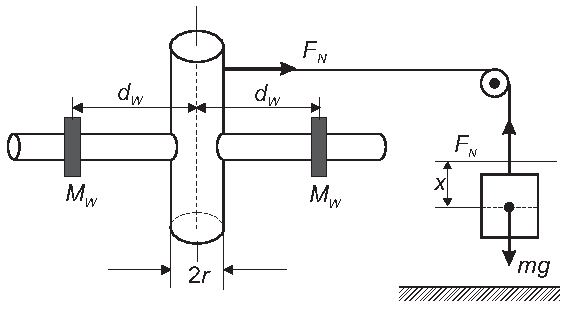
\includegraphics [width=0.95\columnwidth] {img/m7-schemat.pdf}
  \caption{\small
  Schemat układu doświadczalnego z wahadłem Oberbecka.
  Źródło: I~Pracownia Fizyczna, \emph{Badanie ruchu obrotowego bryły sztywnej (M7)}, Instytut Fizyki~UJ~\cite{pracownia-fizyczna-m7}.
  }
  \label{fig:schemat-m7}
\end{figure}

\begin{figure}
  \centering
  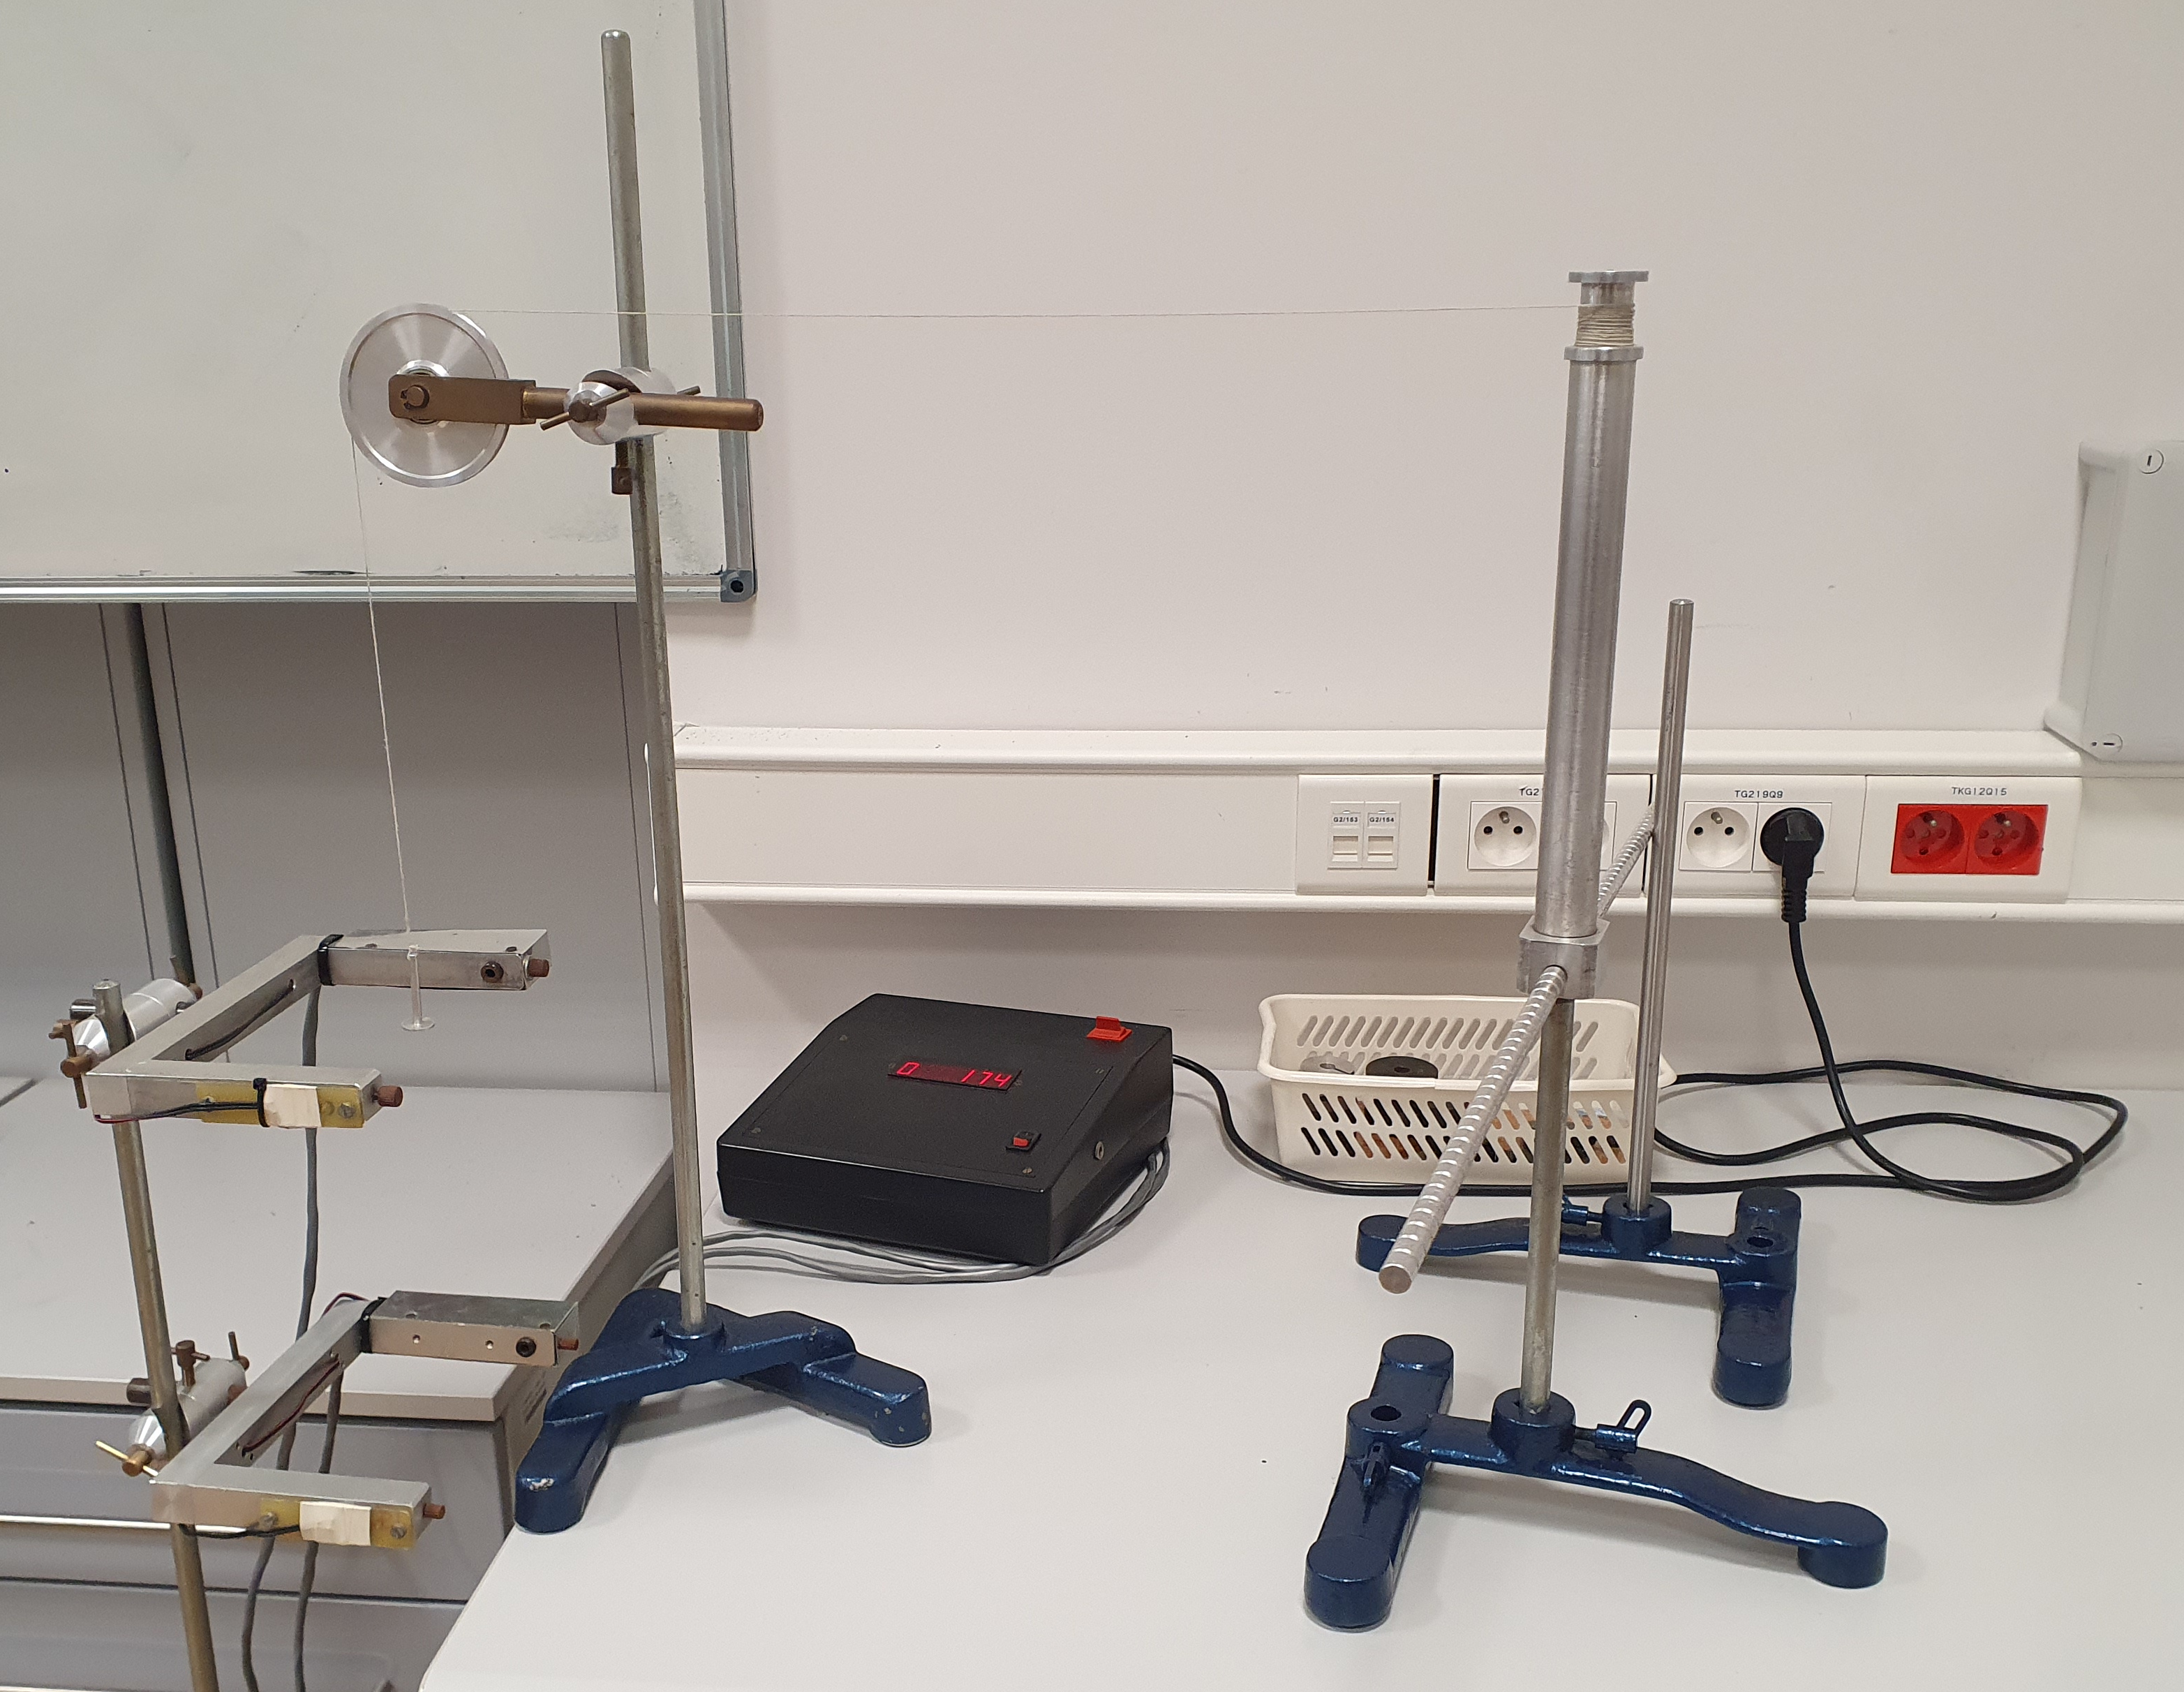
\includegraphics [width=0.95\columnwidth] {img/zdjecie-ukladu.jpg}
  \caption{\small Zdjęcie układu pomiarowego z widocznym Wahadłem Oberbecka oraz bramkami elektronicznymi służącymi do pomiaru czasu.}
  \label{fig:zdjecie-ukladu}
\end{figure}

\section{Przebieg pomiarów}
Dla każdej z trzech badanych zależności wykonanych zostało 5 serii pomiarowych.
Każda seria składała się z 10 pomiarów czasu.

Ze względu na bardzo wysoką precyzję bramki elektronicznej (systematyczna niepewność graniczna wynosi $10^{-3}~\mathrm{s}$) oraz stosunkowo sporą niepewność statystyczną serii pomiarów: $\ge 3.2 \cdot 10^{-2}~\mathrm{s}$, za niepewność pomiarów czasu posłużyła jedynie niepewność statystyczna.

Wielokrotne pomiary długości przy pomocy suwmiarki oraz miary zwijanej dawały za każdym razem takie same wyniki.
Tak samo było dla pomiarów masy przy użyciu wagi laboratoryjnej.
Z tego względu za niepewności długości oraz masy posłużą wspomniane w poprzednim rozdziale niepewności systematyczne.

\section{Wyniki i dyskusja}
\subsection{Regresja liniowa}
Dla każdej z trzech badanych zależności została dopasowana prosta do danych pomiarowych przy użyciu regresji liniowej.
W każdym przypadku wartości szukanej funkcji liniowej odpowiadają kwadratowi czasu $t^2$.
Wzór (\ref{eq:niepewnosc-t-kwadrat}) na niepewność kwadratu czasu $u(t^2)$ uzyskany został przy pomocy zależności (\ref{eq:propagacja-niepewnosci-1-zmienna}).
\begin{equation}
    u(t^2) = 2\bar{t}~u(t)
    \label{eq:niepewnosc-t-kwadrat}
\end{equation}

Regresja liniowa przeprowadzona została w programie \textit{OriginLab} \footnote{\url{https://www.originlab.com/}}.
Ze względu na różne wartości niepewności wartości $t^2$, użyta została regresja ważona w wariancie \textit{Instrumental}.
Waga $w_i$ danego punktu pomiarowego $(x_i, y_i)$ jest dana jako $w_i = \left( u(y_i) \right)^{-2}$ \cite{origin-fitting-weighting}.

\subsection{Parametry stałe wahadła}
\label{sec:parametry-stale-wahadla}
Promień, na którym siła naciągu linki generuje moment siły, jest w rozważaniach teoretycznych niezmienny.
W praktyce dokładna wartość tego promienia jest trudna do zmierzenia, gdyż linka czasem nawinięta jest bezpośrednio na metalowy walec, a czasem sama tworzy dodatkową pełną warstwę znacząco zwiększającą promień.
Wartość promienia $r$ została więc oszacowana jako średnia pomiędzy tymi dwoma sytuacjami.
Do niepewności granicznej pomiaru promienia wahadła dodana została połowa grubość linki, gdyż w danym pomiarze nie wiadomo jak akurat linka się ułożyła.
Otrzymana została wartość (\ref{eq:wahadlo-promien}).
\begin{equation}
    r = 8.00(58)~\mathrm{mm}
    \label{eq:wahadlo-promien}
\end{equation}

\subsection{Przyspieszenie ziemskie}
Jako przyspieszenie ziemskie na terenie Krakowa przyjmujemy wartość (\ref{eq:przyspieszenie-ziemskie}) \cite{przyspieszenie-ziemskie-krakow}.
\begin{equation}
    g = 9.8100(5)~\mathrm{\frac{m}{s^2}}
    \label{eq:przyspieszenie-ziemskie}
\end{equation}

\subsection{Zależność I: \texorpdfstring{$t^2$}{t²} od \texorpdfstring{$h$}{h}}
\subsubsection{Pomiary}
Ciężarek zawieszony na linie podczas badania tej zależności miał masę o wartości (\ref{eq:zaleznosc-i-masa}).
\begin{equation}
    m = 32.20(12)~g
    \label{eq:zaleznosc-i-masa}
\end{equation}

Wyniki pomiarów $h$ i $t$ dla zależności I oraz obliczony kwadrat czasu $t^2$ wraz z niepewnością przedstawione są w Tabeli \ref{tab:zaleznosc-i}.
\begin{table}[ht]
\begin{center}
\renewcommand*{\tablename}{Tabela}
\caption{\small Wyniki pomiarów: wysokość $h$ przebyta przez ciężarek, średni zmierzony czas $t$ z niepewnością oraz obliczony kwadrat czasu $\bar{t}^2$ wraz z niepewnością.\vspace{0.15cm}
    \label{tab:zaleznosc-i}}
    {\small
    \begin{tabular}{c c r r}
    \hline \vspace{-0.35cm} \\
      Lp.
      & $h~[\mathrm{cm}]$ & $\bar{t}~[\mathrm{s}]$ & $\bar{t}^2~[\mathrm{s^2}]$ \\ 
      \hline \vspace{-0.2cm} \\
     1 & 17.3 & 6.2(1) & 38(2) \\
     2 & 31.7 & 9.0(2) & 81(2) \\
     3 & 46.0 & 11.2(1) & 126(3) \\
     4 & 65.1 & 13.3(2) & 177(3) \\
     5 & 85.5 & 15.4(2) & 238(5) \\
    \hline
    \end{tabular}}
    \end{center}
\end{table}

\subsubsection{Regresja liniowa}
W wyniku regresji liniowej uzyskane zostały parametry prostej o wartościach~(\ref{eq:regresja-i-parametry}).
\begin{equation}
\begin{split}
    a &= (294.1 \pm 4.3)~\mathrm{ s^2 m^{-1} } \\
    b &= (-12.3 \pm 1.7)~\mathrm{s^2}
    \label{eq:regresja-i-parametry}
\end{split}
\end{equation}

Miara dopasowania $R^2$ ma wartość: $R^2 = 0.99937$, co spełnia warunek dopasowania krzywej w regresji $R^2 \geq 0.99$ \cite{epa-8000d}.
Na szczególną uwagę zasługuje fakt, że oczekiwana w rozważaniach teoretycznych zerowa wartość wyrazu wolnego prostej (wzór \ref{eq:zaleznosc-i}) nie mieści się w przedziale ufności $3 u(b)$, co pokazuje wzór (\ref{eq:regresja-i-przedzial-ufnosci-b}).
Może to sugerować rozbieżność, między rozważaniami teoretycznymi, a realiami układu doświadczalnego.
\begin{equation}
\begin{split}
    0 &\notin \left( -17.2, -7.5 \right)~\mathrm{s^2} \\
    &\approx \left( \bar{b} - 3 u(b), \bar{b} + 3 u(b) \right)
    \label{eq:regresja-i-przedzial-ufnosci-b}
\end{split}
\end{equation}

Dane z Tabeli \ref{tab:zaleznosc-i} wraz z dopasowaną krzywą o parametrach (\ref{eq:regresja-i-parametry}) zostały zaprezentowane na Rysunku~\ref{img:regresja-i-wykres}.
\begin{figure}[ht]
    \centering

    \begin{tikzpicture}
        \begin{axis}[
            width=8.4cm, height=7cm,
            xlabel={$h~[\mathrm{cm}]$},
            ylabel={$t^2~[\mathrm{s}^2]$},
            legend pos=north west,
            grid=major,
            legend style={font=\footnotesize}
        ]

        \addlegendimage{only marks, mark=*, blue, mark options={fill=red}, error bars/.cd, y dir=both, y explicit}
        \addlegendentry{Punkty pomiarowe}
        
        \addlegendimage{no markers, red, thick}
        \addlegendentry{Dopasowanie regresji liniowej}
        
        \def\slope{2.9411189}
        \def\intercept{-12.32102}
        
        \addplot [red, thick, domain=15:88, forget plot] {\slope*x + \intercept};
        \addlegendentry{Dopasowanie regresji liniowej}
    
        \addplot+[
            only marks,
            mark=*,
            blue,
            mark options={fill=red},
            forget plot,
            error bars/.cd,
            y dir=both,
            y explicit,
        ] table [x=x, y=y, y error=err] {
            x       y               err
            17.3    38.00106025     1.22030149
            31.7    81.47048121     1.924432727
            46.0    125.5408203     2.062786691
            65.1    176.9033003     2.683325469
            85.5    237.745561      4.544923276
        };
        \addlegendentry{Punkty pomiarowe}
    
        \end{axis}
    \end{tikzpicture}

    \caption{
        Dane pomiarowe dla Zależności II wraz z dopasowaniem regresji liniowej: $t^2(h) = ah + b$. Niepewności $t^2$ są ledwo widoczne na wykresie, niepewności $h$ są na tyle małe, że nie widać ich wcale.}
    \label{img:regresja-i-wykres}
\end{figure}


\subsubsection{Obliczenie momentu bezwładności}
Przy użyciu wzoru (\ref{eq:zaleznosc-i-moment-bezwladnosci}) został wyliczony moment bezwładności nieobciążonego wahadła $\JX$ z zależności I. Wynik przedstawia równanie (\ref{eq:zaleznosc-i-wynik}).
Wykorzystano do tego zmierzone wcześniej wartości: (\ref{eq:wahadlo-promien}), (\ref{eq:przyspieszenie-ziemskie}), (\ref{eq:zaleznosc-i-masa}) oraz (\ref{eq:regresja-i-parametry}). Obliczoną wartość (\ref{eq:zaleznosc-i-wynik}) oznaczamy jako $\JXn{I}$.
\begin{equation}
    \JXn{I} = 2.97(44) \cdot 10^{-3}~\mathrm{kg~m^2}
    \label{eq:zaleznosc-i-wynik}
\end{equation}

Niepewność wyniku (\ref{eq:zaleznosc-i-wynik}) $\JXn{I}$ policzona została przy użyciu wzoru (\ref{eq:propagacja-niepewnosci-wiele-zmiennych}).
Informacja o tym, w jakim stopniu dane składniki wpływają na niepewność wyniku znajduje się w Tabeli~\ref{tab:zaleznosc-i-niepewnosci}.

\begin{table}[ht]
\begin{center}
\renewcommand*{\tablename}{Tabela}
\caption{\small Czynniki wpływające na niepewność pomiaru $\JX$ zależnością I dla każdej wielkości ($x$).\vspace{0.15cm}
    \label{tab:zaleznosc-i-niepewnosci}}
    {\small
    \begin{tabular}{c c l}
    \hline \vspace{-0.35cm} \\
      Lp.
      & $x$
      & $\left( \pdv{\JX}{x} u(x) \right)^2 [kg^2~m^4]$ \\ 
      \hline \vspace{-0.2cm} \\
     1 & $r$ & $1.8 \cdot 10^{-7}$ \\
     2 & $a$ & $1.9 \cdot 10^{-9}$ \\
     3 & $m$ & $4.5 \cdot 10^{-10}$ \\
     4 & $g$ & $2.3 \cdot 10^{-14}$ \\
    \hline
    \end{tabular}}
    \end{center}
\end{table}

\subsection{Zależność II: \texorpdfstring{$t^2$}{t²} od \texorpdfstring{$\dwSq$}{dw²}}
\subsubsection{Pomiary}
Ciężarek zawieszony na linie podczas badania tej zależności miał masę o wartości (\ref{eq:zaleznosc-ii-masa}).
\begin{equation}
    m = 98.50(12)~\mathrm{g}
    \label{eq:zaleznosc-ii-masa}
\end{equation}

Badana wysokość $h$ miała w tym scenariuszu stałą wartość (\ref{eq:zaleznosc-ii-wysokosc}).
\begin{equation}
    h = 19.800(58)~\mathrm{cm}
    \label{eq:zaleznosc-ii-wysokosc}
\end{equation}

Krążki użyte jako dodatkowe obciążenia przy padaniu tej zależności miały masy $M_{\mathrm{W,1}}$ i $M_{\mathrm{W,2}}$, promień $R_{\mathrm{W}}$ oraz wysokość $H_{\mathrm{W}}$ o wartościach (\ref{eq:zaleznosc-ii-parametry-walcow}).
\begin{equation}
\begin{split}
    M_{\mathrm{W,1}} &= 241.80(6)~\mathrm{g} \\
    M_{\mathrm{W,2}} &= 253.00(6)~\mathrm{g} \\ \\
    R_{\mathrm{W}}   &= 2.05(3)~\mathrm{cm} \\
    H_{\mathrm{W}}   &= 1.45(6)~\mathrm{cm}
    \label{eq:zaleznosc-ii-parametry-walcow}
\end{split}
\end{equation}

Wyniki pomiarów $d_{\mathrm{W}}$ i $t$, obliczony kwadrat odległości ułożenia ciężarka $\dwSq$ oraz kwadrat czasu $t^2$ wraz z niepewnościami przedstawione są w Tabeli \ref{tab:zaleznosc-ii}.
\begin{table}[ht]
\begin{center}
\renewcommand*{\tablename}{Tabela}
\caption{\small Wyniki pomiarów $d_{\mathrm{W}}$ i $t$, obliczony kwadrat odległości ułożenia ciężarka $\dwSq$ oraz kwadrat czasu $\bar{t}^2$ wraz z niepewnościami.
Każdy z pomiarów odległości $d_{\mathrm{W}}$ obarczony jest niepewnością $u(d_{\mathrm{W}}) = 0.29~\mathrm{mm}$.\vspace{0.15cm}
    \label{tab:zaleznosc-ii}}
    {\small
    \begin{tabular}{c c r r r}
    \hline \vspace{-0.35cm} \\
      Lp.
      & $d_{\mathrm{W}}~[\mathrm{dm}]$ & $\dwSq~[\mathrm{dm^2}]$
      & $\bar{t}~[\mathrm{s}]$ & $\bar{t}^2~[\mathrm{s^2}]$ \\ 
      \hline \vspace{-0.2cm} \\
      1 & 0.32 & 0.099(2) & 4.06(7) & 16.5(6) \\
      2 & 1.01 & 1.020(6) & 5.86(5) & 34.4(6) \\
      3 & 1.71 & 2.92(1) & 8.32(6) & 69(2) \\
      4 & 2.41 & 5.81(2) & 11.3(2) & 126(3) \\
      5 & 2.82 & 7.95(2) & 12.7(2) & 162(4) \\
   
    \hline
    \end{tabular}}
    \end{center}
\end{table}

\subsubsection{Regresja liniowa}
W wyniku regresji liniowej uzyskane zostały parametry prostej o wartościach~(\ref{eq:regresja-ii-parametry}).
\begin{equation}
\begin{split}
    a &= 1.880(24) \cdot 10^3~\mathrm{ s^2 m^{-2} } \\
    b &= 14.85(37)~\mathrm{s^2}
    \label{eq:regresja-ii-parametry}
\end{split}
\end{equation}

Miara dopasowania $R^2$ ma wartość: $R^2 = 0.99953$, co spełnia warunek dobrego dopasowania krzywej w regresji $R^2 \geq 0.99$ \cite{epa-8000d}.
Dane z Tabeli \ref{tab:zaleznosc-ii} wraz z dopasowaną krzywą o parametrach (\ref{eq:regresja-ii-parametry}) zostały zaprezentowane na Rysunku~\ref{img:regresja-ii-wykres}.
\begin{figure}[ht]
    \centering

    \begin{tikzpicture}
        \begin{axis}[
            width=8.4cm, height=7cm,
            xlabel={$\dwSq~[\mathrm{dm^2}]$},
            ylabel={$t^2~[\mathrm{s}^2]$},
            legend pos=north west,
            grid=major,
            legend style={font=\footnotesize}
        ]

        \addlegendimage{only marks, mark=*, blue, mark options={fill=red}, error bars/.cd, y dir=both, y explicit}
        \addlegendentry{Punkty pomiarowe}
        
        \addlegendimage{no markers, red, thick}
        \addlegendentry{Dopasowanie regresji liniowej}
        
        \def\slope{18.7965233}
        \def\intercept{14.8481}
        
        \addplot [red, thick, domain=-0.1:8.1, forget plot] {\slope*x + \intercept};
        \addlegendentry{Dopasowanie regresji liniowej}
    
        \addplot+[
            only marks,
            mark=*,
            blue,
            mark options={fill=red},
            forget plot,
            error bars/.cd,
            y dir=both,
            y explicit,
        ] table [x=x, y=y, y error=err] {
            x           y               err
            7.9524      162.027441      4.061729736
            0.099225    16.45356969     0.5661758554
            2.9241      69.26899984     1.080984169
            1.0201      34.39001449     0.5575028803
            5.8081      126.4680176     3.259685309
        };
        \addlegendentry{Punkty pomiarowe}
    
        \end{axis}
    \end{tikzpicture}

    \caption{
        Dane pomiarowe dla Zależności II wraz z dopasowaniem regresji liniowej: $t^2(\dwSq) = a~\dwSq + b$. Niepewności $t^2$ są ledwo widoczne na wykresie, niepewności $\dwSq$ są na tyle małe, że nie widać ich wcale.
    }
    \label{img:regresja-ii-wykres}
\end{figure}


Wyrażenie (\ref{eq:zaleznosc-ii-parametr-a}) pozwala nam teraz skontrolować zgodność uzyskanej prostej z wartością oczekiwaną w rozważaniach teoretycznych $a_{\mathrm{T}}$, której wartość przedstawia równość (\ref{eq:regresja-ii-a-teoretyczne}).
\begin{equation}
\begin{split}
    a_{\mathrm{T}} = 2 \frac{h \MWS}{m g r^2} = 3.05(44) \cdot 10^3~\mathrm{ s^2 m^{-2} }
    \label{eq:regresja-ii-a-teoretyczne}
\end{split}
\end{equation}

Wartość współczynnika kierunkowego $a$ uzyskanego w regresji liniowej mieści się jedynie w przedziale ufności $3u(a_{\mathrm{T}})$, co obrazuje zależność (\ref{eq:regresja-ii-przedzial-ufnosci-a}).
Fakt, że potrzebny jest przeciał ufności $3u(a_{\mathrm{T}})$ może być kolejną sugestią istnienia rozbieżności między założeniami teoretycznymi, a rzeczywistością.
\begin{equation}
\begin{split}
    a &= 1.880(24) \cdot 10^3~\mathrm{ s^2 m^{-2} } \\
    &\in \left( 1.73, 4.38 \right) 10^3~\mathrm{ s^2 m^{-2} } \\
    &\approx \left(
        \bar{a_{\mathrm{T}}} - 3 u(a_{\mathrm{T}}),
        \bar{a_{\mathrm{T}}} + 3 u(a_{\mathrm{T}})
    \right)
    \label{eq:regresja-ii-przedzial-ufnosci-a}
\end{split}
\end{equation}

\subsubsection{Obliczenie momentu bezwładności}
Przy użyciu wzoru (\ref{eq:zaleznosc-ii-moment-bezwladnosci}) został wyliczony moment bezwładności wahadła bez obciążenia $\JX$ z zależności II.
Wykorzystano do tego zmierzone wcześniej wartości: (\ref{eq:wahadlo-promien}), (\ref{eq:przyspieszenie-ziemskie}), (\ref{eq:zaleznosc-ii-masa}) (\ref{eq:zaleznosc-ii-wysokosc}) (\ref{eq:zaleznosc-ii-parametry-walcow}) oraz (\ref{eq:regresja-ii-parametry}). Wynik przedstawia równanie (\ref{eq:zaleznosc-ii-wynik}). Obliczoną wartość oznaczamy jako $\JXn{II}$.
Niepewność wyniku policzona została przy użyciu wzoru (\ref{eq:propagacja-niepewnosci-wiele-zmiennych}).
\begin{equation}
    \JXn{II} = 2.25(34) \cdot 10^{-3}~\mathrm{kg~m^2}
    \label{eq:zaleznosc-ii-wynik}
\end{equation}

\subsection{Zależność III: \texorpdfstring{$t^2$}{t²} od \texorpdfstring{$m^{-1}$}{1/m}}
\subsubsection{Pomiary}
Badana wysokość $h$ miała stałą wartość (\ref{eq:zaleznosc-iii-wysokosc}).
\begin{equation}
    h = 19.800(58)~\mathrm{cm}
    \label{eq:zaleznosc-iii-wysokosc}
\end{equation}

Wyniki pomiarów masy ciężarków $m$ i czasu $\bar{t}$, obliczona odwrotność masy $m^{-1}$ oraz kwadrat czasu $\bar{t}^2$ wraz z niepewnościami przedstawione są w Tabeli \ref{tab:zaleznosc-iii}.
\begin{table}[ht]
\begin{center}
\renewcommand*{\tablename}{Tabela}
\caption{\small Wyniki pomiarów masy ciężarków $m$ i czasu $\bar{t}$, obliczona odwrotność masy $m^{-1}$ oraz kwadrat czasu $\bar{t}^2$ wraz z niepewnościami.
Każdy z pomiarów masy $m$ obarczony jest niepewnością $u(m) = 58~\mathrm{mg}$.\vspace{0.15cm}
    \label{tab:zaleznosc-iii}}
    {\small
    \begin{tabular}{c l r r r}
    \hline \vspace{-0.35cm} \\
      Lp.
      & $m~[\mathrm{g}]$ & $m^{-1}~[\mathrm{kg^{-1}}]$
      & $\bar{t}~[\mathrm{s}]$ & $\bar{t}^2~[\mathrm{s^2}]$ \\
      \hline \vspace{-0.2cm} \\
      1 & 197 & 5.076(3) & 2.80(3) & 7.9(2) \\
      2 & 147 & 6.812(5) & 3.20(3) & 10.3(2) \\
      3 & 98.5 & 10.15(2) & 3.81(6) & 14.5(5) \\
      4 & 60.3 & 16.58(3) & 5.02(8) & 25.2(8) \\
      5 & 12.1 & 82.6(8) & 11.2(2) & 126(3) \\
    
\hline
    \end{tabular}}
    \end{center}
\end{table}

\subsubsection{Regresja liniowa}
W wyniku regresji liniowej uzyskane zostały parametry prostej o wartościach~(\ref{eq:regresja-iii-parametry}).
\begin{equation}
\begin{split}
    a &= 1.500(35)~\mathrm{ s^2 kg } \\
    b &= 0.09(27)~\mathrm{s^2}
    \label{eq:regresja-iii-parametry}
\end{split}
\end{equation}

Miara dopasowania $R^2$ ma wartość: $R^2 = 0.99923$, co spełnia warunek dobrego dopasowania krzywej w regresji $R^2 \geq 0.99$ \cite{epa-8000d}.
Dane z Tabeli \ref{tab:zaleznosc-iii} wraz z dopasowaną krzywą o parametrach (\ref{eq:regresja-iii-parametry}) zostały zaprezentowane na Rysunku~\ref{img:regresja-iii-wykres}.
\begin{figure}[ht]
    \centering

    \begin{tikzpicture}
        \begin{axis}[
            width=8.4cm, height=7cm,
            xlabel={$\dwSq~[\mathrm{dm^2}]$},
            ylabel={$t^2~[\mathrm{s}^2]$},
            legend pos=north west,
            grid=major,
            legend style={font=\footnotesize}
        ]

        \addlegendimage{only marks, mark=*, blue, mark options={fill=red}, error bars/.cd, y dir=both, y explicit}
        \addlegendentry{Punkty pomiarowe}
        
        \addlegendimage{no markers, red, thick}
        \addlegendentry{Dopasowanie regresji liniowej}
        
        \def\slope{1.50007}
        \def\intercept{0.08968}
        
        \addplot [red, thick, domain=3:85, forget plot] {\slope*x + \intercept};
        \addlegendentry{Dopasowanie regresji liniowej}
    
        \addplot+[
            only marks,
            mark=*,
            blue,
            mark options={fill=red},
            forget plot,
            error bars/.cd,
            y dir=both,
            y explicit,
        ] table [x=x, y=y, y error=err] {
            x               y               err            
            10.15228426     14.52295881     0.4577332822   
            5.076142132     7.85456676      0.1789283481   
            82.6446281      125.6102978     2.581700008    
            16.58374793     25.17229584     0.7899873803   
            6.811989101     10.26817936     0.1653895391   
        };;
        \addlegendentry{Punkty pomiarowe}
    
        \end{axis}
    \end{tikzpicture}

    \caption{
        Dane pomiarowe dla Zależności III wraz z dopasowaniem regresji liniowej: $t^2(m^{-1}) = a~m^{-1} + b$. Niepewności $t^2$ są ledwo widoczne na wykresie, niepewności $m^{-1}$ są na tyle małe, że nie widać ich wcale.
    }
    \label{img:regresja-iii-wykres}
\end{figure}


Wyrażenie (\ref{eq:zaleznosc-iii-parametr-b}) pozwala nam teraz skontrolować zgodność uzyskanej prostej z wartością oczekiwaną w rozważaniach teoretycznych.
$b_{\mathrm{T}}$ to teoretyczna wartość wyrazu wolnego prostej, której wartość przedstawia równość (\ref{eq:regresja-iii-b-teoretyczne}).
\begin{equation}
\begin{split}
    b_{\mathrm{T}} = \frac{2h}{g} = 0.04036(11)~\mathrm{s^2}
    \label{eq:regresja-iii-b-teoretyczne}
\end{split}
\end{equation}

Wartość teoretycznego wyrazu wolnego prostej mieści się w przedziale ufności $1u(b)$, co obrazuje zależność~(\ref{eq:regresja-iii-przedzial-ufnosci-b}).
\begin{equation}
\begin{split}
    b_{\mathrm{T}} &= 0.04036(11)~\mathrm{s^2} \\
    &\in \left( -0.18, 0.36 \right)~\mathrm{s^2} \\
    &\approx \left(
        \bar{b} - u(b),
        \bar{b} + u(b)
    \right)
    \label{eq:regresja-iii-przedzial-ufnosci-b}
\end{split}
\end{equation}

\subsubsection{Obliczenie momentu bezwładności}
Przy użyciu wzoru (\ref{eq:zaleznosc-iii-moment-bezwladnosci}) został wyliczony moment bezwładności wahadła bez obciążenia $\JX$ z zależności III. Wynik przedstawia równanie (\ref{eq:zaleznosc-iii-wynik}).
Wykorzystano do tego zmierzone wcześniej wartości: (\ref{eq:wahadlo-promien}), (\ref{eq:przyspieszenie-ziemskie}), (\ref{eq:zaleznosc-iii-wysokosc}) oraz (\ref{eq:regresja-iii-parametry}). Obliczoną wartość oznaczamy jako $\JXn{III}$.
\begin{equation}
    \JXn{III} = 2.38(35) \cdot 10^{-3}~\mathrm{kg~m^2}
    \label{eq:zaleznosc-iii-wynik}
\end{equation}

\subsection{Uproszone szacowanie momentu bezwładności wahadła}
Aby oszacować moment bezwładności nieobciążonego wahadła poprzez potraktowanie go jako walec obracający się względem osi prostopadłej do osi symetrii obrotowej, potrzebne są dodatkowe pomiary.
Długość pręta przyczepionego do wahadła oznaczymy przez $l_{\mathrm{P}}$, natomiast jego promień przez $r_{\mathrm{P}}$. Wielkości te mają wartości~(\ref{eq:parametry-preta}).
\begin{equation}
\begin{split}
    l_{\mathrm{P}} &= 62.100(58)~\mathrm{cm} \\
    r_{\mathrm{P}} &= 5.00(29)~\mathrm{mm} 
    \label{eq:parametry-preta}
\end{split}
\end{equation}

Wykorzystując wzór~(\ref{eq:moment-bezwladnosci-preta}), zmierzone parametry~(\ref{eq:parametry-preta}) pręta oraz wartość~(\ref{eq:aluminium-gestosc}) gęstości aluminium, jesteśmy w stanie oszacować moment bezwładności wahadła $\JXn{Sz}$ traktując je jako walec.
Wartość~(\ref{eq:wartosc-moment-bezwladnosci-preta}) przedstawia uzyskany rezultat.
\begin{equation}
    \JXn{Sz} = 4.23(49) \cdot 10^{-3}~\mathrm{kg~m^2}
    \label{eq:wartosc-moment-bezwladnosci-preta}
\end{equation}

\section{Podsumowanie i wnioski}
\subsection{Ocena dopasowania modelu}
Współczynnik korelacji $R^2$ dla każdej z 3 wykonanych regresji liniowych wyniósł $R^2 \ge 0.999$, co spełnia warunek dobrego dopasowania krzywej w regresji $R^2 \geq 0.99$ \cite{epa-8000d}.
Stwierdzona liniowość badanych wielkości potwierdza słuszność praw ruchu obrotowego.

\subsection{Oczekiwane teoretyczne współczynniki prostych}
Zastanawiającym jest fakt, że w Zależności I oczekiwany w założeniach teoretycznych zerowy wyraz wolny funkcji liniowej $b$ nie był zawarty w przedziale ufności $3u(b)$ uzyskanych parametrów dopasowanej prostej.
Podobny problem wystąpił w Zależności II, jednak tam uzyskana wartość współczynnika kierunkowego prostej $a$ mieściła się w przedziale ufności $3u(a_{\mathrm{T}})$ oczekiwanej wartości teoretycznej.
Jako przyczynę takiego stanu rzeczy wskazałbym fakt, że układ nie spełnia wszystkich kryteriów zakładanych przez rozważania teoretyczne.
Dla przykładu bloczek zmieniający kierunek działania siły naciągu linki sam posiada niezerową bezwładność, co nie zostało ujęte w założeniach teoretycznych.
Dodatkowym założeniem, które prawdopodobnie nie zostało spełnione, jest zerowa prędkość ciężarka w momencie rozpoczęcia pomiaru czasu.
Dość spora rozbieżność pomiarów czasu w ramach serii pomiarowych (rzędu $1$~s) sugeruje, że warunek ten nie był spełniony dla sporej części pomiarów.
Taki wniosek powodowałby, że wartość średnia pomiarów czasu w ramach serii nie jest w rzeczywistości najbardziej prawdopodobną \enquote{prawdziwną} wartością, a jest on niej większa.

\subsection{Źródło niepewności otrzymanego wyniku}
Głównym źródłem niepewności otrzymanych wyników nie okazało się dopasowanie prostej przy pomocy regresji liniowej, a niepewność pomiaru promienia, na którym siła naciągu linki działa jako moment siły przyspieszający cały układ.
Zostało to dokładniej opisane w Podrozdziale \ref{sec:parametry-stale-wahadla}.
Dodatkowym źródłem niepewności była błędna obsługa suwmiarki, co uwidacznia przyjęty błąd pomiarowy.

W celu zmniejszenia niepewności uzyskanych wyników dobrym pomysłem mogłoby się okazać powtórzenie pomiarów suwmiarką, tak aby wyniki były obarczone najmniejszą niepewnością, na jaki pozwala przyrząd.
Innym pomysłem na zmniejszenie niepewności mogłoby być zmodyfikowanie wahadła tak, aby mierzony promień miał bardziej przewidywalną i większą wartość.

\subsection{Porównanie otrzymanych wyników}
Uzyskane momenty bezwładności dla każdej z trzech zależności oraz wartość oszacowana zostały zebrane w Tabeli~\ref{tab:porownanie-wynikow}.
\begin{table}[ht]
\begin{center}
\renewcommand*{\tablename}{Tabela}
\caption{\small
Zebrane uzyskane momenty bezwładności dla każdej z trzech zależności oraz wartość oszacowana wraz z niepewnościami.
\vspace{0.15cm}
    \label{tab:porownanie-wynikow}}
    {\small
    \begin{tabular}{l r}
    \hline \vspace{-0.35cm} \\
      Metoda & $10^{-3} \JX~\mathrm{kg~m^2}$ \\
      \hline \vspace{-0.2cm} \\
      Zależność I & 2.97(44) \\
      Zależność II & 2.25(34) \\
      Zależność III & 2.38(35) \\
      Szacowanie & 4.23(49) \\
    \hline
    \end{tabular}}
    \end{center}
\end{table}

W celu lepszej wizualizacji narysowany został Rysunek~\ref{img:gestosc-prawdop-porownanie} przedstawiający funkcje gęstości prawdopodobieństwa dla rozkładów wszystkich uzyskanych wartości momentów bezwładności.
Zaznaczone zostały także wartości oczekiwane.
\begin{figure}[ht]
    \centering
    \begin{tikzpicture}
        \begin{axis}[
            width=8.2cm, height=7cm,
            xlabel={$10^{-3} J \, [kg \, m^2]$},
            ylabel={Gęstość prawdopodobieństwa},
            grid=major,
            scaled x ticks=false,
            x tick label style={/pgf/number format/fixed, /pgf/number format/precision=4},
            legend style={at={(1.00,1.00)}, anchor=north east, font=\footnotesize}
        ]

        % --- Zaleznosc I ---
        \def\muOne{2.97}
        \def\sigmaOne{0.44}

        % --- Zaleznosc II ---
        \def\muTwo{2.25}
        \def\sigmaTwo{0.34}

        % --- Zaleznosc III ---
        \def\muThree{2.38}
        \def\sigmaThree{0.35}

        % --- Szacowanie ---
        \def\muFour{4.23}
        \def\sigmaFour{0.49}

        \def\medium{3}
        \def\range{1.5}

        % --- Zaleznosc I ---
        \addplot [
            domain=\medium - \range : \medium + \range,
            samples=1000,
            color=red,
            thick,
            smooth
        ]
        {1/(\sigmaOne*sqrt(2*pi)) * exp(-((x-\muOne)^2)/(2*\sigmaOne^2))};
        \addlegendentry{Zależność I}

        % --- Zaleznosc II ---
        \addplot [
            domain=\medium - \range : \medium + \range,
            samples=1000,
            color=blue,
            thick,
            smooth
        ]
        {1/(\sigmaTwo*sqrt(2*pi)) * exp(-((x-\muTwo)^2)/(2*\sigmaTwo^2))};
        \addlegendentry{Zależność II}

        % --- Zaleznosc III ---
        \addplot [
            domain=\medium - \range : \medium + \range,
            samples=1000,
            color=green,
            thick,
            smooth
        ]
        {1/(\sigmaThree*sqrt(2*pi)) * exp(-((x-\muThree)^2)/(2*\sigmaThree^2))};
        \addlegendentry{Zależność III}

        % --- Szacowanie ---
        \addplot [
            domain=\medium - \range : \medium + \range,
            samples=1000,
            color=purple,
            thick,
            smooth
        ]
        {1/(\sigmaFour*sqrt(2*pi)) * exp(-((x-\muFour)^2)/(2*\sigmaFour^2))};
        \addlegendentry{Szacowanie}

        % --- Punkty --- %
        \pgfmathsetmacro{\peakOne}{1/(\sigmaOne*sqrt(2*pi))}
        \draw [dashed, red!70] (axis cs:\muOne, 0) -- (axis cs:\muOne, \peakOne);
        \addplot[mark=*, mark size=1.5pt, red] coordinates {(\muOne, \peakOne)};
        \addplot[mark=*, mark size=1.5pt, red] coordinates {(\muOne, 0)};
        
        \pgfmathsetmacro{\peakTwo}{1/(\sigmaTwo*sqrt(2*pi))}
        \draw [dashed, blue!70] (axis cs:\muTwo, 0) -- (axis cs:\muTwo, \peakTwo);
        \addplot[mark=*, mark size=1.5pt, blue] coordinates {(\muTwo, \peakTwo)};
        \addplot[mark=*, mark size=1.5pt, blue] coordinates {(\muTwo, 0)};

        \pgfmathsetmacro{\peakThree}{1/(\sigmaThree*sqrt(2*pi))}
        \draw [dashed, green!70] (axis cs:\muThree, 0) -- (axis cs:\muThree, \peakThree);
        \addplot[mark=*, mark size=1.5pt, green] coordinates {(\muThree, \peakThree)};
        \addplot[mark=*, mark size=1.5pt, green] coordinates {(\muThree, 0)};
        
        \pgfmathsetmacro{\peakFour}{1/(\sigmaFour*sqrt(2*pi))}
        \draw [dashed, purple!70] (axis cs:\muFour, 0) -- (axis cs:\muFour, \peakFour);
        \addplot[mark=*, mark size=1.5pt, purple] coordinates {(\muFour, \peakFour)};
        \addplot[mark=*, mark size=1.5pt, purple] coordinates {(\muFour, 0)};

        \end{axis}
    \end{tikzpicture}
    \caption{Porównanie gęstości prawdopodobieństwa uzyskanych momentów bezwładności dla każdej z trzech metod wraz z zaznaczonymi wartościami oczekiwanymi.}
    \label{img:gestosc-prawdop-porownanie}
\end{figure}


Z wykresu: Rysunek~\ref{img:gestosc-prawdop-porownanie} można zauważyć, że Zależność II oraz III dały niemalże identyczne wyniki.
Zależność I dostarczyła nieco większej wartości momentu bezwładności, jednakże wartości oczekiwane dla dwóch kolejnych zależności $(\bar{\JXn{II}}, \bar{\JXn{III}})$ mieszczą się w przedziale ufności $2u(\JXn{I})$.
Na uwagę zasługuje znacznie większy rezultat momentu bezwładności oszacowanego poprzez podobieństwo wahadła do walca.
Co ciekawe, rezultat jest większy od pozostałych wartości, a nie mniejszy, jak można by oczekiwać.
Wahadło z układu to nie jest jedynie poprzeczny aluminiowy pręt, który został przybliżony walcem, lecz także pusty w środku pręt podłużny.
Pomimo że jego masa znajduje się blisko środka ciężkości, należałoby się spodziewać, że w sposób zauważalny zwiększy bezwładność całości.

\section{Materiały dodatkowe}
\subsection{Konwersja niepewności granicznej na niepewność standardową}
Dla dowolnej mierzonej wielkości $X$ jej niepewność graniczną $\Delta X$ można skonwertować na niepewność standardową $u(X)$ przy pomocy wzoru (\ref{eq:konwersja-niepewnosci}) \cite{smop-wyklad}.
\begin{equation}
    u(X) = \frac{ \Delta X }{ \sqrt{3} }
    \label{eq:konwersja-niepewnosci}
\end{equation}

\subsection{Propagacja niepewności funkcji jednej zmiennej}
Dla dowolnej mierzonej wielkości $X$ niepewność standardową funkcji tej wielkości $u(~f(X)~)$ można policzyć przy użyciu wzoru (\ref{eq:propagacja-niepewnosci-1-zmienna}) \cite{smop-wyklad}.
\begin{equation}
    u( f(X) ) = \dv{f(X)}{X} u(X)
    \label{eq:propagacja-niepewnosci-1-zmienna}
\end{equation}

\subsection{Propagacja niepewności funkcji wielu zmiennych}
Niepewność standardową wartości $Y$, będącą wartością funkcji wielu zmiennych $(X_1, X_2, \dots, X_n)$ można policzyć przy użyciu wzoru (\ref{eq:propagacja-niepewnosci-wiele-zmiennych}) \cite{smop-wyklad}.
\begin{equation}
    u(Y) = \sqrt{ \sum_{i=1}^n \left( \pdv{Y}{X_i} u(X_i) \right)^2 }
    \label{eq:propagacja-niepewnosci-wiele-zmiennych}
\end{equation}

\section{Podziękowania}
Dziękuję Pani dr Magdalenie Skalskiej za cenne dyskusje i opiekę podczas przeprowadzenia eksperymentu.

\begin{thebibliography}{7}
    \bibitem{epa-8000d} US Environmental Protection Agency (EPA), \emph{Method 8000D: Determinative Chromatographic Separations}, (\url{https://www.epa.gov/sites/default/files/2015-12/documents/8000d.pdf}) (dostęp:~21.03.2026).

    \bibitem{przyspieszenie-ziemskie-krakow} \emph{Dziennik normalizacji i miar nr 13/81 r.}, Polski Komitet Normalizacji, Miar i Jakości (\url{https://www.gum.gov.pl/download/2/1854/dzienniknormalizacjiimiar198113.pdf}).

    \bibitem{pracownia-fizyczna-m7} I~Pracownia Fizyczna, \emph{Badanie ruchu obrotowego bryły sztywnej (M7)}, Instytut Fizyki~UJ (\url{https://1pf.if.uj.edu.pl/materialy-do-cwiczen/spis-cwiczen}) (dostęp:~15.03.2026).

    \bibitem{smop-wyklad} dr~hab. \mbox{Katarzyna} \mbox{Gajos}, Wykład \emph{Statystyczne Metody Opracowania Pomiarów I Dla studentów fizyki}.

    \bibitem{origin-fitting-weighting} OriginLab Corporation, \emph{Origin Help}, rozdział \textbf{15.3.6.5} \emph{Fitting with Errors and Weighting} (\url{https://www.originlab.com/doc/Origin-Help/FIt-with-Err-Weight}) (dostęp:~21.03.2026).
    
    \bibitem{oberbeck-wiki}Wikipedia, \emph{Anton Oberbeck}, (\url{https://en.wikipedia.org/wiki/Anton_Oberbeck}) (dostęp:~15.03.2026).
\end{thebibliography}

\end{document}
